\section{Bài 07}

(Absence of KKT points) Xem xét bài toán
\begin{equation}
    \label{problem:07}
    \begin{aligned}
        \min \quad & x^2 + y^2\\
        \textrm{s.t.} \quad & x^2 - (y - 1)^3 = 0\\
    \end{aligned}
\end{equation}

\begin{enumerate}[label=(\alph*)]
    \item Giải bài toán này theo phương pháp hình học.
    \item Chứng minh rằng không tồn tại điểm nào thỏa mãn điều kiện KKT.
    \item Tìm tất cả các điểm thỏa mãn điều kiện FJ.
    \item Khi thử giải bài toán tối ưu bằng cách thế ngược $x^2 = (y - 1)^3$ trong hàm mục tiêu, do đó giảm thiểu nó về bài toán không ràng buộc:
    \begin{equation}
        \begin{aligned}
            \min \quad & y^2 + (y-1)^3\\
        \end{aligned}
    \end{equation}
    Những có điều gì đó chưa đúng với phương pháp này. Đó là gì, và làm thế nào để hiệu chỉnh lại cho đúng.
\end{enumerate}

\begin{solution}

    Các thành phần trong bài toán này như sau:
    \begin{align}
        \begin{aligned}
            f(x,y) &= x^2 + y^2\\
            h_1(x,y) &= x^2 - (y - 1)^3\\
        \end{aligned}
    \end{align}
    \begin{enumerate}[label=(\alph*)]
    \item Giải bài toán này theo phương pháp hình học.
    \begin{figure}[h!]
        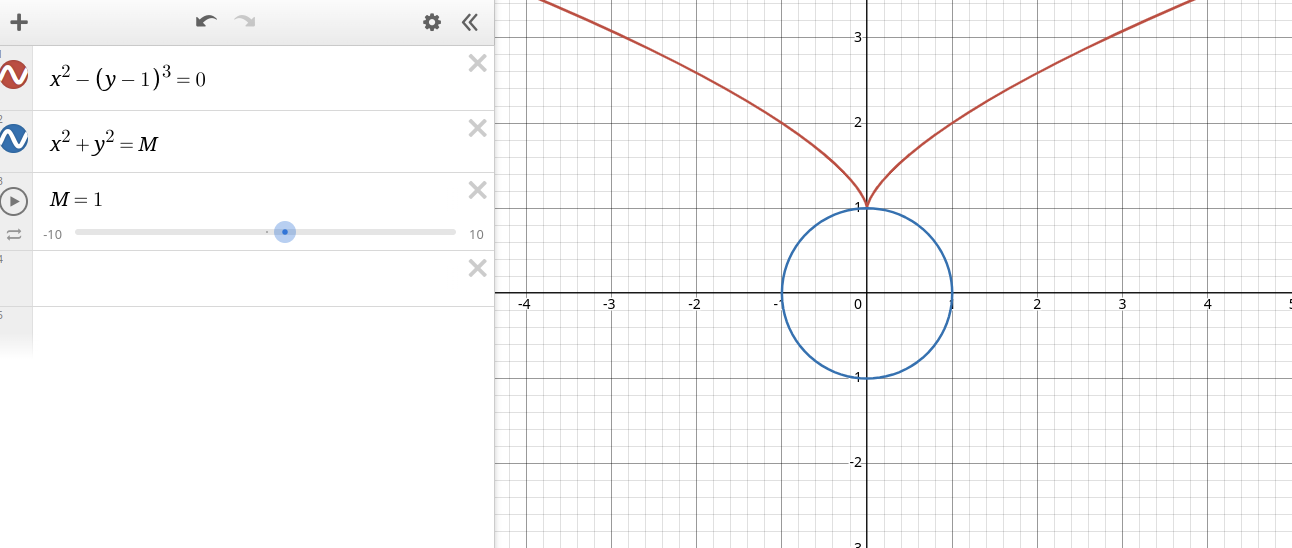
\includegraphics[width=0.85\linewidth]{figures/BT07.png}
        \caption{Miền khả thi của bài toán (\ref{problem:07}).}
        \label{fig:feasible_region_problem_03}
    \end{figure}
    \item Chứng minh rằng không tồn tại điểm nào thỏa mãn điều kiện KKT. Ta có dạng hàm Lagrangian như sau:
    \begin{equation}
        L(x, y, \mu) = x^2 + y^2 + \mu_1\left[x^2 - (y - 1)^3\right]
    \end{equation}
    và các điều kiện KKT được viết như sau:
    \begin{itemize}
        \item \begin{equation}
            \dfrac{\partial L}{\partial x} = 2x + 2\mu_1x = 0 \Leftrightarrow \begin{cases}
                x = 0\\ 
                \text{hoặc} \\
                \mu_1 = -1
            \end{cases}
        \end{equation}
        \item \begin{equation}
            \dfrac{\partial L}{\partial y} = 2y - 3\mu_1(y-1)^2 = 0
        \end{equation}
        \item \begin{equation}
            x^2 - (y - 1)^3 = 0
        \end{equation}
    \end{itemize}
    Nếu $x = 0$ thì 
    \begin{equation}
        \begin{cases}
            y = 1\\
            \mu_1 = t, t \in \R
        \end{cases}
    \end{equation} thì $(x, y) = (0,1)$ không thỏa điều kiện KKT vì không thể xác định được $\mu_1$.
    Nếu $\mu_1 = -1$ thì
    \begin{equation}
        \begin{cases}
            2y + 3(y-1)^2 = 0\\
            x^2 - (y-1)^2 = 0
        \end{cases}
    \end{equation}
    thì hệ này vô nghiệm.
    Vậy, ta không tìm được điểm KKT nào.
    \item Tìm tất cả các điểm thỏa mãn điều kiện FJ. Ta có dạng yếu của hàm Lagrangian như sau:
    \begin{equation}
        L(x, y, \lambda, \mu) = \lambda_0(x^2 + y^2) + \mu_1\left[x^2 - (y - 1)^3\right]
    \end{equation}
    và các điều kiện FJ được viết như sau:
    \begin{itemize}
        \item \begin{equation}
            \dfrac{\partial L}{\partial x} = 2\lambda_0x + 2\mu_1x = 0 \Leftrightarrow \begin{cases}
                x = 0\\ 
                \text{hoặc} \\
                \mu_1 = -\lambda_0
            \end{cases}
        \end{equation}
        \item \begin{equation}
            \dfrac{\partial L}{\partial y} = 2\lambda_0y - 3\mu_1(y-1)^2 = 0
        \end{equation}
        \item \begin{equation}
            x^2 - (y - 1)^3 = 0
        \end{equation}
    \end{itemize}
    Nếu $x = 0$ thì 
    \begin{equation}
        \begin{cases}
            y = 1\\
            \lambda_0 = 0\\
            \mu_1 = t, t \in \R
        \end{cases}
    \end{equation}
     thì hệ này có nghiệm $(x, y) = (0,1)$
     Nếu $\mu_1 = -\lambda_0$ thì
    \begin{equation}
        \begin{cases}
            2\lambda_0y - 3\lambda_0(y-1)^2 = 0\\
            x^2 - (y-1)^2 = 0
        \end{cases}
        \Leftrightarrow
        \begin{cases}
            \lambda_0 \ne 0 \\ 
            y = \dfrac{4+\sqrt{7}}{3}\quad\text{hoặc}\quad y = \dfrac{4-\sqrt{7}}{3} \\\\
            x = \sqrt{\left(\dfrac{1+\sqrt{7}}{3}\right)}\quad\text{hoặc}\quad x = -\sqrt{\left(\dfrac{1+\sqrt{7}}{3}\right)}
        \end{cases}
    \end{equation}
    Vậy các điểm FJ lần lượt là:
    \begin{equation}
        \left(\sqrt{\left(\dfrac{1+\sqrt{7}}{3}\right)}, \dfrac{4+\sqrt{7}}{3}\right); \left(-\sqrt{\left(\dfrac{1+\sqrt{7}}{3}\right)}, \dfrac{4-\sqrt{7}}{3}\right)
    \end{equation}
    \item Khi thử giải bài toán tối ưu bằng cách thế ngược $x^2 = (y - 1)^3$ trong hàm mục tiêu, do đó giảm thiểu nó về bài toán không ràng buộc:
    \begin{equation}
        \begin{aligned}
            \min \quad & y^2 + (y-1)^3\\
        \end{aligned}
    \end{equation}
    Những có điều gì đó chưa đúng với phương pháp này. Đó là gì, và làm thế nào để hiệu chỉnh lại cho đúng. 

    Ta thấy nếu $x^2 - (y - 1)^3 = 0$ thì ta phải có $y \geq 1$. Đây là một ràng buộc ẩn và nó sẽ biến mất nếu ta thay thế $x^2 = (y - 1)^2$ trong hàm mục tiêu. Nếu ta loại bỏ $x$, ta phải đảm bảo rằng $y \geq 1$. Nếu ta không thêm vào ràng buộc này, thì hàm mục tiểu $y^2 + (y-1)^3$ sẽ không bị chặn.
\end{enumerate}
\end{solution}